% \documentclass[11pt,a4paper,uplatex,twoside,dvipdfmx]{ujarticle} 	% for uplatex
% \documentclass[11pt,a4paper,twoside,dvipdfmx]{jarticle}		% platex
\documentclass[11pt,a4paper,twoside,dvipdfmx]{jsarticle}   % 美文書
%==== 科研費LaTeX =============================================
%	2020(H32)年度 PD
%============================================================
% 2008-03-08: Taku Yamanaka (JSPS Research Center for Science Systems / Osaka Univ.)
% 2008-03-10: Taku; Fixed a bug which was missing p.7.
% 2009-03-04: K.S.: Revised for JFY2010.
% 2010-03-04: Taku: Revised for JFY2011.
% 2011-03-20: Taku: Revised for JFY2012.
% 2012-02-25: Taku: Revised for JFY2013.
% 2013-03-14: Taku: Revised for JFY2014.
% 2014-03-02: Taku: Revised for JFY2015.
% 2015-02-23: Taku: Revised for JFY2016.
% 2016-02-26: Taku: Revised for JFY2017.
%============================================================
%=======================================
% form00_header.tex
%	General header for kakenhiLaTeX,  Moved over from form00_2010_header.tex.
%	2009-09-06 Taku Yamanaka (Osaka Univ.)
%==== General Version History ======================================
% 2006-05-30 Taku Yamanaka (Physics Dept., Osaka Univ.)
% 2006-06-02 V1.0
% 2006-06-14 V1.1 Use automatic calculation for cost tables.
% 2006-06-18 V1.2 Split user's contents and the format.
% 2006-06-20 V1.3 Reorganized user and format files
% 2006-06-25 V1.4 Readjusted all the table column widths with p{...}.
%				With \KLTabR and \KLTabRNum, now the items can be right-justified
%				in the cell defined by p{...}.
% 2006-06-26 V1.5 Use \newlength and \setlength, instead of \newcommand, to define positions.
% 2006-08-19 V1.6 Remade it for 2007 JFY version.
% 2006-09-05 V1.7 Added font declarations suggested by Hoshino@Meisei Univ.
% 2006-09-06 V1.8 Introduced usePDFform flag to switch the form file format.
% 2006-09-09 V1.9 Changed p.7, to allow different heights between years. (Thanks to Ytow.)
% 2006-09-11 V2.0 Added an option to show budget summary.
% 2006-09-13 V2.1 Added an option to show the group.
% 2006-09-14 V2.1.1 Cleaned up Kenkyush Chosho.
% 2006-09-21 V2.2 Generated under a new automatic development system.

% 2007-03-24 V3.0 Switched to a method using "picture" environment.

% 2007-08-14 V3.1 Switched to kakenhi3.sty.
% 2007-09-17 V3.2 Added \KLMaxYearCount
% 2008-03-08 V3.3 Remade it for 2009 JFY version\
% 2008-09-08 V3.4 Added \KLXf ... \KLXh.
% 2011-10-20 V5.0 Use kakenhi5.sty, to utilize array package in tabular environment.
% 2012-08-14 v5.1 Moved preamble and kakenhi5 into the current directory, instead of the parent directory.
% 2012-11-10 v6.0 Switched to kakenhi6.sty.
% 2015-08-26 v6.1 Added KLFirstPageIsLongPage flag.
% 2018-02-12 Taku: Commented out \DeclareFontShape ...
%=======================================
%============================================================
% preamble.tex
%
% Dummy section and subsection commands.
% With these, some editors (such as TeXShop, etc.) can jump to the (sub)sections.
\newcommand{\dummy}{dummy}% 
\renewcommand{\section}[1]{\renewcommand{\dummy}{#1}}
\renewcommand{\subsection}[1]{\renewcommand{\dummy}{#1}}

% Flag for switching form file format.......
\usepackage{ifthen}
\newboolean{usePDFform}
\newboolean{BudgetSummary}

\usepackage{forms/kakenhi6}

\pagestyle{empty}

% ===== Parameters for LaTeX =========================

% ===== Font declarations  ======================================
%%\DeclareFontShape{JT1}{mc}{m}{it}{<->ssub * mc/m/n}{}
%%\DeclareFontShape{JY1}{mc}{m}{it}{<->ssub * mc/m/n}{}

% ===== Parameters for KL (Kakenhi LaTeX) ========================
% general purpose temporary variables	-2007
\newcommand{\KLX}{}
\newcommand{\KLXa}{}
\newcommand{\KLXb}{}
\newcommand{\KLXc}{}
\newcommand{\KLXd}{}
\newcommand{\KLXe}{}
\newcommand{\KLXf}{}
\newcommand{\KLXg}{}
\newcommand{\KLXh}{}
\newcommand{\KLY}{}
\newcommand{\KLYa}{}
\newcommand{\KLYb}{}
\newcommand{\KLYc}{}
\newcommand{\KLYd}{}
\newcommand{\KLYe}{}
\newcommand{\KLYf}{}
\newcommand{\KLXR}{}
\newlength{\KLCella}
\newlength{\KLCellb}
\newlength{\KLCellc}
\newlength{\KLCelld}
\newlength{\KLCelle}
\newlength{\KLCellf}
\newlength{\KLCellg}
\newlength{\KLCellh}

% sub-page
\newlength{\KLSubPageX}
\newlength{\KLSubPageY}
\newlength{\KLspx}
\newlength{\KLspy}
\newcommand{\KLSubPageXmm}{}	% for \input(x,y){....} which uses a unit (mm)
\newcommand{\KLSubPageYmm}{}	% for \input(x,y){....} which uses a unit (mm)

% margins for parbox inside frames; in units of points
\newcounter{KLParboxSideMargin}
\newcounter{KLParboxTopMargin}
\newcounter{KLParboxBottomMargin}

% ===== standard counters ======================================
\newcounter{KLSubPageNo}	% sub-page counter
\newcounter{KLPageOffset}		% to generate sub-page number
\newcounter{KLMaxYearCount}	% # of years for the proposal

% ===== standard flags ============================
\newboolean{KLFirstPageIsLongPage}

% ===== initializations ============
\KLInitTypesettingPageSelection
\newcommand{\KLCLLang}{}	% language-dependent left-justification in tabular



% user01_header
%=== 様式のファイルの形式の指定 =================
%   PDFではなく、eps の様式を読み込む場合は、次の行の頭に「%」をつけてください。
\setboolean{usePDFform}{true}
%===================================
%==========================================================
% form01_header.tex
%	2014-03-02: Taku Yamanaka (Osaka Univ.)
%		This is called after usePDFform is set.
%		Originally, this part was in form07_header.tex, but then
%		\usepackage{color} that is called before it was not effective.
%		[dvipdfmx] is not used for eps forms, because it makes the forms
%		slightly larger than pdf forms.
%		
%==========================================================
% ===== File format for forms ===========================
\ifthenelse{\boolean{usePDFform}}{
	\newcommand{\KLFormFormat}{pdf}	\usepackage[dvipdfmx]{graphicx}
}{	\newcommand{\KLFormFormat}{eps}	\usepackage{graphicx}
}

%----------------------------------------------------------------------------


% user02_header
%=== 予算の表の印刷 =====================
% 予算の集計の表を出すためには、次の行の頭の%を消してください。
%\setboolean{BudgetSummary}{true}
%=================================

%=== For English, uncomment the next line to left-justify inside table columns.
%\renewcommand{\KLCLLang}{\KLCL}

% === 一部のページだけタイプセット ==============
% New in 2009 fall version!
% 選んだページだけタイプセットするには、次の例の頭の%を消し、並べてください。
% 複数のページを選ぶこともできます。
% 提出前には、必ず全てコメントアウト(頭に%をつける)してください。
%ーーーーーーーーーーーーーーーーーーーーーーーーーーーーーーーーー
%\KLTypesetPage{1}			% p.1 (or p.1を含む連続したページ),
%\KLTypesetPage{3}			% p.3 (or p.3を含む連続したページ),
%\KLTypesetPagesInRange{5}{6}	% p.5 ~ p.6,
%\KLTypesetPagesInRange{8}{10}	% and p.8 ~ p.10
%=================================

% ===== my favorite packages ====================================
% ここに、自分の使いたいパッケージを宣言して下さい。
\usepackage{wrapfig}
% \usepackage{amssymb}
%\usepackage{mb}
\usepackage[usenames]{color} % でも科研費の書類はグレースケールで印刷されます
\usepackage{udline}
\usepackage{amsmath,amssymb}
\usepackage[expert,deluxe]{otf}
\usepackage{setspace}
%\DeclareGraphicsRule{.tif}{png}{.png}{`convert #1 `dirname #1`/`basename #1 .tif`.png}
%==========================================================

\newcommand{\KLShouKeiLine}[1]{\cline{#1}}
%もし、小計の上の線を取れと事務に言われたら、
%「そのようなことは、記入要項に書かれていないし、学振はそのようなことは気にしていない。」と
% 突っぱねる。
% それでもなお消せと理不尽なことを言われたら、次の行の 最初の「%」を消す。	
%\renewcommand{\KLShouKeiLine}[1]{}

\newcommand{\KLBudgetTableFontSize}{small}	% 予算の表のフォントの大きさ: small, footnotesize
\newcommand{\KLFundsTableFontSize}{small}	%応募中、受入れ予定の研究費のフォントの大きさ:normalsize, small, footnotesize

% ===== my personal definitions ==================================
% ここに、自分のよく使う記号などを定義して下さい。
\setlength {\fboxrule}{1pt} % 箱の枠線の太さを変える
\setlength {\fboxsep}{3pt} % 箱枠内側の余白幅を変える
\definecolor{my_gray}{gray}{0.9}
\def\rem#1{ {\bf\textcolor{red}{($\clubsuit$ #1 $\clubsuit$)}}}
\renewcommand{\emph}[1]{{\usekanji{JY1}{hgt}{bx}{n} #1}}

\let\oldenumerate\enumerate
\renewcommand{\enumerate}{
\oldenumerate
\setlength{\itemsep}{1.2pt}
\setlength{\parskip}{0pt}
\setlength{\parsep}{0pt}
}

% hook3: after including packages ===================
 % for future maintenance
% ===== Global definitions for the PD form ======================
% 基本情報
%
%------ 研究課題名  -------------------------------------------
\newcommand{\研究課題名}{粒子加速器を用いた電弱相互作用を持つ新物理の探索}

%----- 研究機関名と研究代表者の氏名-----------------------
\newcommand{\研究機関名}{東京大学}
\newcommand{\申請者氏名}{千草颯}
\newcommand{\研究代表者氏名}{\申請者氏名}

%---- 研究期間の最終年度 ----------------
\newcommand{\研究期間の最終元号年度}{34}	%平成で、半角数字のみ
%=========================================================
% ===== Global year-dependent definitions for the Kakenhi form ===========
% 基本情報
\newcommand{\研究開始年度}{2020}
\newcommand{\研究開始元号年度}{32}	%平成

\newcommand{\1年目西暦}{2020}
\newcommand{\2年目西暦}{2021}
\newcommand{\3年目西暦}{2022}
\newcommand{\4年目西暦}{2023}
\newcommand{\5年目西暦}{2024}
\newcommand{\6年目西暦}{2025}

\newcommand{\1年目}{32}
\newcommand{\2年目}{33}
\newcommand{\3年目}{34}
\newcommand{\4年目}{35}
\newcommand{\5年目}{36}
\newcommand{\6年目}{37}

\newcommand{\1年目J}{32}
\newcommand{\2年目J}{33}
\newcommand{\3年目J}{34}
\newcommand{\4年目J}{35}
\newcommand{\5年目J}{36}
\newcommand{\6年目J}{37}


	% 
%==========================================================
% form03_header.tex
%	2009-03-04: Taku Yamanaka (Osaka Univ.)
%==========================================================
\usepackage{calc}
\usepackage{watermark}
\usepackage{longtable}
\usepackage{geometry}                % See geometry.pdf to learn the layout options. There are lots.
\usepackage{udline}
\usepackage{array}

\geometry{noheadfoot,scale=1}  %scale=1 resets margins to 0
\setlength{\unitlength}{1pt}

% define variables for positions ==========================
% picture environment location, in  units of points
\newcommand{\KLOddPictureX}{}
\newcommand{\KLEvenPictureX}{}
\newcommand{\KLPictureY}{}
\newcommand{\KLOddPictureInWaterMarkX}{}
\newcommand{\KLEvenPictureInWaterMarkX}{}
\newcommand{\KLPictureInWaterMarkY}{}

\newlength{\KLoddsidemargin}
\newlength{\KLevensidemargin}
\newlength{\KLtopmargin}

\newcounter{KLCOddPictureInWaterMarkX}
\newcounter{KLCEvenPictureInWaterMarkX}
\newcounter{KLCPictureInWaterMarkY}
\newcounter{KLCOddPictureX}
\newcounter{KLCEvenPictureX}
\newcounter{KLCPictureY}

%------------------------------------------------------------

\newcommand{\KLLeftEdge}{}
\newcommand{\KLRightEdge}{}

% standard margins for text in frames
\setcounter{KLParboxSideMargin}{7}
\setcounter{KLParboxTopMargin}{12}
\setcounter{KLParboxBottomMargin}{5}

%-----------------------------------------------------------
\newcommand{\KLTwoHLines}{\hline\hline}



%=================================================================
% form05_pd_header.tex
%	for the 2007(H19) Japanese Fiscal Year
%	2006-10-01 : Taku Yamanaka (Osaka Univ.)
%			Switched to the new development system using a "mother file".
%	2007-08-08: Taku
%			Switched to a new method using "picture" environment.
%	2008-03-08: Taku
%			Readjusted parameters for the new 2008 form.
%	2009-09-04: Taku
%			Introduced form03_header and form07_header to automatically calculate margins and
%			other miscellaneous coordinate parameters.
%=================================================================

% ===== Global definitions for the Kakenhi form ======================
% 基本情報
\newcommand{\研究種目}{PD}
\newcommand{\研究種目後半}{}
\ifthenelse{\isundefined{\研究種別}}{
	\newcommand{\研究種別}{}
}{}%
\newcommand{\KLMainFile}{pd.tex}
\newcommand{\KLForms}{pd_forms}
\newcommand{\KLYoshiki}{pd}

% 奇数ページの下に記入される情報
\newcommand{\klbyYup}{}
\newcommand{\klbyYdown}{}
\newcommand{\klbyKikanXleft}{}
\newcommand{\klbyKikanXright}{}
\newcommand{\klbyNameXleft}{}
\newcommand{\klbyNameXright}{}

\newcommand{\KLBottomInfo}[6]{%
	\ifthenelse{\equal{#1}{}}{%
		\renewcommand{\klbyYup}{62}
		\renewcommand{\klbyYdown}{48}
	}{%
		\renewcommand{\klbyYup}{#1}
		\renewcommand{\klbyYdown}{#2}
	}
	
	\ifthenelse{\equal{#3}{}}{%
		\renewcommand{\klbyKikanXleft}{132}
		\renewcommand{\klbyKikanXright}{349}
		\renewcommand{\klbyNameXleft}{425}
		\renewcommand{\klbyNameXright}{550}
	}{%
		\renewcommand{\klbyKikanXleft}{#3}
		\renewcommand{\klbyKikanXright}{#4}
		\renewcommand{\klbyNameXleft}{#5}
		\renewcommand{\klbyNameXright}{#6}
	}
%	\KLTextBox{\klbyKikanXleft}{\klbyYup}{\klbyKikanXright}{\klbyYdown}{}{\研究機関名}%
	\KLTextBox{\klbyNameXleft}{\klbyYup}{\klbyNameXright}{\klbyYdown}{}{\申請者氏名}%
}

%==========================================================
% frame edge positions of multi-page-block
\newcommand{\KLOddMultiPageLeftEdge}{47}
\newcommand{\KLOddMultiPageRightEdge}{549}
\newcommand{\KLEvenMultiPageLeftEdge}{47}
\newcommand{\KLEvenMultiPageRightEdge}{549}

% vertical limits in the first multi-page-block
\newcommand{\KLMultiPageTopEdge}{806}		%lowest top position (except for the 1st page)
\newcommand{\KLMultiPageBottomEdge}{80}	%highest bottom position (except for the last page)

% Modify the edges for single page frames if necessary
\newcommand{\KLOddLeftEdge}{\KLOddMultiPageLeftEdge}
\newcommand{\KLOddRightEdge}{\KLOddMultiPageRightEdge}
\newcommand{\KLEvenLeftEdge}{\KLEvenMultiPageLeftEdge}
\newcommand{\KLEvenRightEdge}{\KLEvenMultiPageRightEdge}

%

%==========================================================
% form07_header.tex
%	2009-03-04: Taku Yamanaka (Osaka Univ.)
%	2014-03-02: Taku: Moved graphics part to form01_header.tex.
%	2015-08-26: Taku: Added a test for \KLFirstPageIsLongPage.
%==========================================================
% Remember Standard Positions that were set in form05_xxxx_header.tex
\let \KLStandardOddMultiPageLeftEdge = \KLOddMultiPageLeftEdge
\let \KLStandardOddMultiPageRightEdge = \KLOddMultiPageRightEdge
\let \KLStandardEvenMultiPageLeftEdge = \KLEvenMultiPageLeftEdge
\let \KLStandardEvenMultiPageRightEdge = \KLEvenMultiPageRightEdge

\let \KLStandardMultiPageTopEdge = \KLMultiPageTopEdge
\let \KLStandardMultiPageBottomEdge = \KLMultiPageBottomEdge

\let \KLStandardOddLeftEdge = \KLOddLeftEdge
\let \KLStandardOddRightEdge = \KLOddRightEdge
\let \KLStandardEvenLeftEdge = \KLEvenLeftEdge
\let \KLStandardEvenRightEdge = \KLEvenRightEdge

%------ This should be set before \begin{document} ------
\KLStandardLengths
\KLStandardPositions

\ifthenelse{\boolean{KLFirstPageIsLongPage}}{%
	\setlength{\textheight}{10000pt}%
}{%
}
%----------------------------------------------------------------------------


%============================================================
%endPrelude

\usepackage{bm}	% required for `\bm' (yatex added)
\begin{document}
\fontsize{11pt}{17pt}\selectfont
% hook5 : right after \begin{document} ==============
 % for future maintenance
%============================================================
%     User Inputs
%============================================================

%form: pd_form_03-04.tex ; user: pd_03-04_preparation_etc.tex
%========== PD =========
%===== p. 03-04 現在までの研究状況 =============
\section{現在までの研究状況}
%watermark: w03_past_pd
\newcommand{\現在までの研究状況}{%
%begin  現在までの研究状況===================

\noindent{\fcolorbox{black}{my_gray}{これまでの研究の背景、問題点、解決方策}}

% \vspace*{1mm}

\emph{【背景】}2012年に世界最大の加速器施設であるLHCがHiggs粒子を発見
し[1]、素粒子の標準模型が予言する粒子全ての存在が確認された。一方、標
準模型で説明が出来ない現象は多数残されており、宇宙の大半を占める
\emph{暗黒物質の正体}はその代表例である。こうした状況を受けて、加速器
実験では様々な角度から新物理の兆候を探しているが、その中で最も重要な視
点の一つが、\emph{電弱相互作用を持つ新粒子の探索}である。

この視点が重要である理由として、\emph{電弱相互作用を持つ暗黒物質の候補}が
多く存在し、その質量として現在の加速器実験のエネルギーに近いテラスケー
ルの値が予言されることが挙げられる。このような新粒子は現在の暗黒物質残
存量を正しく説明できる上[2]、理論的に興味深い種々の新物理模型とも相性
が良いため、様々な研究に登場する。
%%
また、\emph{高エネルギー領域における電弱相互作用の検証が未だ不十分であ
る}ことも理由の一つである。近年の実験技術の向上により、電弱相互作用の
破れのスケールを超えた領域での精密測定実験が可能となりつつあり、これに
よりテラスケール新粒子の兆候が見られると期待できる。このような実験状況
を鑑みて、新粒子の探索手法を理論的に確立することは火急の課題である。
%%
さらに、加速器実験でHiggsの質量が測定されたことにより、標準模型の真空
は準安定に過ぎないことが明らかとなったが[3]、電弱相互作用を持つ新粒子
は\emph{電弱真空の安定性}へ影響を与えるため、慎重に考慮する必要がある。
%%
以上に挙げたような理由から、電弱相互作用を持つ新粒子の研究は、現代の素
粒子物理学の非常に重要な課題である。

\emph{【問題点】}問題点は \emph{\ul{電弱相互作用を持つ新粒子の探索手法
が十分に確立されていない}} ことである。電弱相互作用が非常に弱い相互作
用であり、観測が容易でないことがその原因である。そのため素粒子理論の知
識を用いて実験結果へのアプローチを工夫し、新粒子の小さな信号を抜き出す
手法を考案する必要がある。

\emph{【解決方策】}電弱相互作用を持った新粒子を探索する上で、高エネル
ギー領域に直接到達可能な粒子加速器による実験を用いることは重要である。
特にここでは、\ul{(1a)特徴的な信号を用いた新物理探索}、および \ul{(1b)
標準模型の過程の精密測定}といった手法でこの問題に取り組む。また、加速
器実験のデータを元に \ul{(2)理論的な考察から新物理の模型を探索する} こ
とも高エネルギー領域へのアプローチとして有用である。次の項目で、
(1a)(1b)(2)それぞれのアプローチについてより具体的に説明する。

\vspace*{1mm}

\noindent{\fcolorbox{black}{my_gray}{研究目的、方法}(詳細は「これまでの研究結果」も参照)}

% \vspace*{1mm}

全体の研究目的は、電弱相互作用を持つ種々の新粒子に対して、粒子加速器を
用いてそれらを発見し、その背後にある物理模型を検証することである。申請
者はこれまで、将来の運営が計画されている \ul{【A】
{$100\,\mathrm{TeV}$} 粒子加速器を用いた新粒子の探索}、および \ul{【B】
Higgs の性質を用いた新物理模型の検証} に着目し、上記の問題に取り組んだ。
以下に、それぞれの研究の目的、および方法について具体的に述べる。

\noindent{■ \emph{\ul{{\textbf{【A】100 TeV}} 粒子加速器を用いた新物理の探索}}(解決方策の(1a)(1b)に対応)}

\vspace*{1mm}

\emph{【背景】}陽子を衝突させる$100\,\mathrm{TeV}$ 粒子加速器の実験で
は、陽子の構成要素であるクォーク間に働く強い相互作用に起因する背景事象
が、観測される事象の圧倒的多数を占めることが予想される。この背景事象の
中から新物理の弱い相互作用に起因する効果を抜き出すためには、実験手法を
工夫する必要がある。

\emph{【目的、方法】}目的は、電弱相互作用を持つ新粒子に高い感度を持つ
実験手法を提案し、新粒子の検出能力を明らかにすることである。以下に、用
いた2つの手法\textbf{(a)(b)}を具体的に説明する。
%%
\textbf{(a)}電磁力の電荷を持つ長寿命粒子が存在すると、これが検出器内を
ある程度の距離飛んだ後崩壊することで、\emph{消失飛跡}と呼ばれる特徴的
な信号を残す。これを用いて、背景事象の数を減らし長寿命粒子への感度を高
められる[4]。ここでは特に、超対称模型の一種であるアノマリー伝搬模型(以
下AMSB模型と表記)に着目する。AMSB模型では、最も軽い新粒子Winoの荷電成
分が長寿命であるため、この手法が強力である。
%%
\textbf{(b)}電弱相互作用の電荷を持つ新粒子が存在すると、量子補正の形で
レプトン対生成過程に影響を与えるが、その際のイベント数への効果はレプト
ン不変質量の関数として\emph{特徴的なピークを持つ}ことが知られている[5]。
レプトン対生成過程の精密測定を行い、理論的に得られるピーク構造の関数形
を用いてデータをフィットすることで、膨大な背景事象から新粒子の情報を抜
き出すことが出来る。
%%
\textbf{(a)(b)}いずれについても、粒子の衝突、崩壊、検出過程をシミュレー
トし、適切な統計的処理を行ってデータを解析する。

\noindent{■ \emph{\ul{{\textbf{【B】Higgs}} の性質を用いた新物理模型の検証}}(解決方策の(2)に対応)}

\vspace*{1mm}

\emph{【背景】}LHCにおいてHiggsが発見され、その質量や結合の強さなども高
精度で測定されている。これらの性質を元に理論的考察を行うことで、電弱相互
作用の構造に関する情報が得られると期待される。

\emph{【目的、方法】}目的は、実験で測定されたHiggsの性質との整合性から、
素粒子模型を検証することである。ここでは特に、Higgs質量の測定により可
能となった、電弱真空の安定性の議論に着目する。具体的には、調べる模型に
対してHiggsの自己相互作用定数に関するくりこみ群方程式を解き、得られた
解を用いて真空崩壊率を評価し、真空の寿命と宇宙の年齢の大小を比較するこ
とで、模型に対する示唆を与える。

\vspace*{1mm}

\noindent{\fcolorbox{black}{my_gray}{これまでの研究結果}}

% \vspace*{1mm}

以下これまでの研究成果をアプローチ毎にまとめる。[4.研究業
績-(1)-3,4,7,8]および[4.研究業績-(6)-2]の全ての研究が博士課程で行った
ものである。\ul{全ての研究で申請者が中心となって解析を行った}。

\noindent{■ \emph{\ul{{\textbf{【ia】}}消失飛跡を用いた新粒子の探索}}(上記 \textbf{【A】} 手法\textbf{(a)}に対応)}

\vspace*{1mm}

AMSB模型に着目し、暗黒物質の有力候補であるWinoの検出可能性を調べた。消
失飛跡の信号を用いることで、暗黒物質残存量から予言される質量を持つWino
が検出できることを明らかにした。また飛跡の速度情報を用いたWino質量の測
定法を与え、測定誤差を見積もった。さらにBinoやgluinoと呼ばれる他の新粒
子のWinoへの崩壊過程を用いて、これらの質量もある程度の誤差で決定できる
ことを示した。質量の測定値を用いた理論的考察から、模型のパラメータの一
部が決定できることを明らかにした[4-(1)-8]。

\noindent{■ \emph{\ul{{\textbf{【ib】}}レプトン対生成過程の精密測定を用いた新物理の探索}}(上記 \textbf{【A】} 手法\textbf{(b)}に対応)}

\vspace*{1mm}

暗黒物質の残存量を正しく予言するような電弱相互作用を持った新粒子の検出
可能性を調べた。超対称模型に含まれるHiggsinoを始めとして、消失飛跡の手
法を適用できない短寿命粒子にこの手法が特に有効で、他の実験手法を凌ぐ検
出能力を与えることを示した[4-(1)-7]。また新物理の寄与が持つピーク構造
の位置や高さから、新物理の質量や電荷などの性質が抜き出せることを示した
[4-(6)-2]。

\noindent{■ \emph{\ul{{\textbf{【ii】}}電弱真空の安定性を用いた素粒子模型の検証}}(上記 \textbf{【B】} に対応)}

\vspace*{1mm}

標準模型と同様、一つのスカラー場が電弱相転移を引き起こす模型に対し、真
空崩壊率を従来より精密に計算するための定式化を与えた。標準模型の場合に
Higgs自己相互作用定数のくりこみ群方程式を解いて真空崩壊率を計算し、電
弱真空の準安定性を再導出した[4-(1)-3]。さらにHiggsと結合する新粒子が存
在する模型で同様の解析を行い、新粒子の質量と結合定数に対する条件式を与
えた[4-(1)-4]。

\vspace*{1mm}

\noindent{\fcolorbox{black}{my_gray}{特色と独創的な点}}(上記\textbf{【A】【B】}それぞれについて記述)

% \vspace*{1mm}

\textbf{【A】}新粒子の信号の特徴を用いたアプローチで、新粒子への感度を
高める点が特色である。また、こういった手法を新物理の性質の決定にまで応
用した文献は少なく、この点が独創的だと言える。

\textbf{【B】}電弱真空の寿命計算における論理的なギャップを埋め、精密計
算を可能にした点が特色である。これを用いてHiggsに結合する新粒子が真空
の寿命に与える影響を計算したのは申請者の研究が初めてであり、この点で独
創的である。また、本研究は Particle Data Group の編纂する素粒子物理の
レビュー論文[6]に引用されており、当該結果が現代素粒子物理学の基礎とな
るようなものであることを示している。

\fontsize{10pt}{13pt}\selectfont
 \underline{参考文献}:
 [1] ATLAS collaboration, Phys. Lett. \textbf{B716} (2012) 1;
 CMS collaboration, Phys. Lett. \textbf{B716} (2012) 30.
 [2] As a recent review, see L. Roszkowski, \textit{et al}., Rept. Prog. Phys. \textbf{81} (2018) 066201.
 [3] G. Degrassi, \textit{et al}., JHEP 1208 (2012) 098.
 [4] S. Masahiko, \textit{et al}., arXiv: 1901.02987 (2019).
 [5] See for example H. Keisuke, \textit{et al}., JHEP 1509 (2015) 105.
 [6] M. Tanabashi, \textit{et al}., Phys. Rev. \textbf{D98} (2018) 030001.

%end  現在までの研究状況 ====================
}

%form: pd_form_05-07.tex ; user: pd_05-07_purpose.tex
%========== PD =========
%===== p. 05-07 これからの研究計画 =============
\section{これからの研究計画}
%watermark: w02_purpose_pd
\subsection{研究の背景}
\newcommand{\研究の背景}{%
%begin  研究の背景===================

\fontsize{11pt}{17pt}\selectfont
\noindent{\fcolorbox{black}{my_gray}{これからの研究計画の背景}}

%%
Higgsの発見により素粒子標準模型は一応の完成を見たが、未だ説明されてい
ない現象は数多く残されており、引き続き様々な角度から新物理の探索が続け
られている。中でも、\emph{高いエネルギー領域における電弱相互作用の検証}を
通じて電弱相互作用を持つ新粒子の兆候を探索することは、近年の実験技術の
向上を鑑みて非常に意義深い。同時に、暗黒物質を説明する模型の多くが電弱
相互作用を持ったテラスケールの新粒子を予言することや、標準模型の電弱真
空は準安定にすぎず、新物理が真空の安定性に与える効果を無視できないこと
などから、電弱相互作用を持つ新粒子の研究は理論的な側面からも重要な課題
である。
%%

\vspace*{1mm}

\noindent{\fcolorbox{black}{my_gray}{問題点と解決すべき点、着想に至った経緯等}}

\vspace*{1mm}

%%
\emph{電弱相互作用を持つ新粒子の探索手法が十分に確立されていない}点が
問題である。申請者の先行研究を含め、こういった新粒子の検出法に関する議
論は近年盛り上がりつつあるが、その背後にある物理模型の理解にまで繋がる手法
は未だ少ない。また精密な寿命計算を元にした電弱真空の安定性の議論は、申
請者の先行研究を含めても数が限られており[3,7]、あらゆる模型で計算が可
能な手法は存在しないのが実情である。

現在もLHCは稼働を続けており、さらに将来実験として$100\,\mathrm{TeV}$加
速器やレプトン加速器等の計画が進められている中、実験結果をどのように活
用すれば新物理模型に対する最大限の知見を得られるかが試されている。申請
者はこういった現状を鑑みた結果、\ul{実験結果へのアプローチを工夫し、理
論的解釈を加えることで、電弱相互作用を持つ新粒子やその背後の物理模型を
探索する}という研究方針を着想するに至った。

% \begin{spacing}{0.8}
\fontsize{10pt}{17pt}\selectfont
\noindent{
 \underline{参考文献}:
 [7] M. Endo, \textit{et al}., JHEP 1711 (2017) 074;
 A. Andreassen, \textit{et al}., Phys. Rev. \textbf{D97} (2018) 056006.
}
% \end{spacing}
%%

%end  研究の背景 ====================
}

\subsection{研究の特色・独創的な点}
\newcommand{\研究の特色と独創的な点}{%
%begin  研究の特色と独創的な点===================

\fontsize{11pt}{17pt}\selectfont

研究全体の特色は、実験結果に対するアプローチを工夫することで、電弱相互
作用を持つ新粒子を探索し、その性質の決定を通じて模型の検証法を与えるこ
とである。

% \vspace*{-1mm}

\noindent{■ \emph{\ul{特色、独創的な点}}}(以下紙面の都合上、[3-(2)研究目的・内容]の\textbf{【I】【II】}について具体的に記述する。)

\vspace*{1mm}

\textbf{【I】}消失飛跡を用いて新粒子を発見するに留まらず、その性質を測
定し、測定結果を用いて新粒子の背後にある根源的な模型を検証する点が独創
的である。

\textbf{【II】}ゲージボソンの崩壊先を太いジェットとしてとらえる手法は、エ
ネルギースケールが高い実験で初めて重要性を帯びるものであり、これを活用し
て解析を行う点が独創的である。またここでの系統誤差の取り扱い方は、あらゆ
る過程や実験セットアップに応用が可能であるという特色を持つ。

\vspace*{-1mm}

\noindent{■ \emph{\ul{位置付け、意義}}}

\vspace*{1mm}
%%
\textbf{【I】}実験結果を元とした理論的考察による模型の検証は、実験自体
のエネルギーよりも遥かに高いエネルギー領域にも言及しうるという点で意義
が大きい。この種の検証が可能な研究は未だ数が限られており、こうした加速
器実験と理論的考察を組み合わせる研究の方向性は発展させていくべきである
と考える。

\textbf{【II】}加速器実験を用いた量子補正の効果の探索は、未だ十分に研
究されておらず、その点で先駆的な研究と言える。一方でこの手法は応用が広
く、手法を確立すること自体に大きな意義がある。
%%

\vspace*{-1mm}

\noindent{■ \emph{\ul{インパクトおよび将来の見通し}}}

\vspace*{1mm}

\textbf{【I】}新粒子の背後にある根源的な模型の検証結果は、素粒子理論の
発展に大きなインパクトを与える。

\textbf{【II】}新しい実験結果が出るに伴い、我々の研究成果を用いてより
強力な素粒子模型の検証が可能となる。また、確立した手法を別の過程にも応
用することで、実験毎に最適な解析を行い、実験から模型の情報を最大限引き
出せる。本研究はこのような将来の発展のための基礎となる。

%end  研究の特色と独創的な点 ====================
}

\subsection{研究目的}
\newcommand{\研究目的}{%
%begin  研究目的===================

% \vspace*{1mm}

\noindent{\fcolorbox{black}{my_gray}{全体の研究目的}}

\vspace*{1mm}
%%
粒子加速器の実験結果への効率的なアプローチを提案することで、電弱相互作
用を持つ新粒子の探索法を与え、さらに理論的考察を通じて背後にある新物理
模型を調査することが研究の目的である。新粒子に対する感度を上げる工夫と
して、まず「I. 消失飛跡を用いた新物理の性質の調査」に着目する。同時に
「II. 標準模型の精密測定を用いた新物理の探索」についても議論する。また
「III. 電弱真空の安定性を用いたより一般の素粒子模型の検証」の研
究も行う。
%%

\begin{wrapfigure}{r}{0.5\textwidth}
 \centering
 % \vspace*{-6mm}
 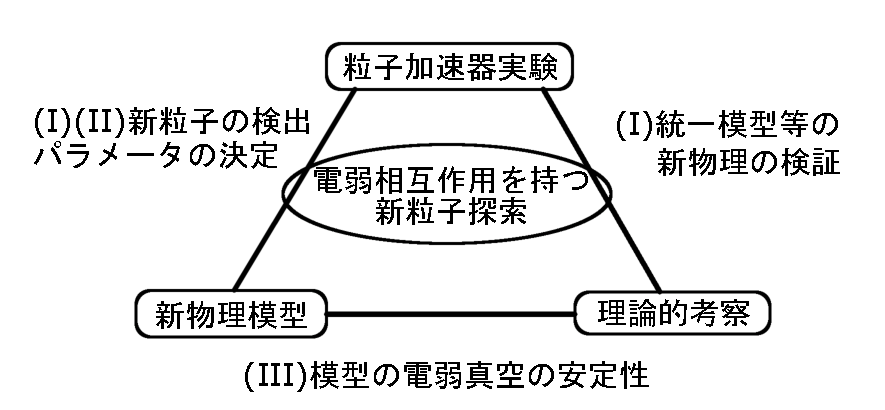
\includegraphics[width=\hsize]{figs/figure.pdf}
 \caption{本研究の全体像}
\end{wrapfigure}

\vspace*{1mm}

\noindent{\fcolorbox{black}{my_gray}{具体的な研究目的と方法、内容}}

\vspace*{1mm}

\noindent{■ \emph{\ul{{\textbf{I.}} 消失飛跡を用いた新物理の性質の調査}}}

\vspace*{1mm}

\noindent{◆ \emph{\ul{研究目的、方法}}}

\vspace*{1mm}

$100\,\mathrm{TeV}$粒子加速器における消失飛跡の信号を用いて、AMSB模型
に加え、その背後にある超対称性の破れのメカニズムや、統一模型などの物理
模型を検証することが目的である。現在までの研究で一部の新粒子の質量の測
定法を与えたが、それに加えて荷電Winoの寿命や、gluinoからBinoもしくは
Winoへの崩壊の分岐比に着目する。

\noindent{\emph{\ul{{\textbf{I-i.}} 長寿命粒子の寿命測定}}}

\vspace*{1mm}

\emph{【背景】}荷電Winoの寿命は質量の関数として詳細に計算されている。一
方、加速器実験における消失飛跡の信号は、一般には長寿命新粒子の存在を示す
のみであり、それをWinoと同一視するためには寿命の情報が必要となる。得ら
れた質量と寿命とを比較することで、AMSB模型の検証が可能となる。

\emph{【内容】}シミュレーションで生成された各荷電Winoに対し、寿命の値
によって定まる確率分布から飛距離を計算し、実験のセットアップと比較する
ことで、何層の検出器を通過したかを調べる。これを実験データとみなし、寿
命の関数としてのイベント数の期待値と比較することで、寿命の決定精度を求
める。質量や寿命の測定誤差を考慮に入れて測定値を理論曲線と比較し、模型
の検証可能性を調査する。

\noindent{\emph{\ul{{\textbf{I-ii.}} {\textbf{gluino}} 崩壊分岐比の測定}}}

\vspace*{1mm}

\emph{【背景】}gluinoからBino、あるいはWinoへの崩壊分岐比は、より重い
クォークの超対称パートナーの質量比によって決定される。実験によって分岐
比が決定されれば、実験の到達範囲を越えたエネルギースケールの物理のヒン
トを得ることができる。この結果は、AMSB模型の背後にある物理模型の検証に
役立つ。

\emph{【内容】}実験でgluinoが生成された場合の信号は、Winoおよび数本の
高エネルギージェットで特徴付けられる。gluinoの崩壊先の違いは高エネルギー
ジェットの本数の違いに対応するが、その他にも過程の途中で多数の低エネル
ギージェットがビーム軸の方向を中心に放出されていると予想されるため、
ジェットの運動量の大きさ、方向に対するカットを工夫し、最も正確に分岐比
を再構成できるカットの条件を調べる。

\noindent{◆ \emph{\ul{展望}}}

\vspace*{1mm}

ここで決定された新物理の性質を元に理論的考察を行うことで、超対称性の破
れのメカニズムや、大統一理論などの統一模型の検証が可能である。また、研
究\textbf{I-ii.}のようなイベントの分類は、教師あり機械学習が得意とする
作業であり、これを用いた解析の改善も視野に入れている。こういった機械学
習の手法は電弱相互作用を持つ新粒子の研究のみならず、粒子加速器実験の解
析一般に応用が可能である。

\noindent{■ \emph{\ul{{\textbf{II.}} 標準模型の精密測定を用いた新物理の探索}}}

\vspace*{1mm}

\noindent{◆ \emph{\ul{研究目的、方法}}}

\vspace*{1mm}

Higgsinoを始めとする電弱相互作用を持つ暗黒物質候補の検出が目的である。
現在までの研究で短寿命Higgsinoに有効な検出法を与えたが、暗黒物質の残存
量から示唆される質量を考えると、検出能力は未だ不十分である。検出能力を
引き上げるため、新たな標準模型過程を解析に加える。また、新粒子の質量が
大きい場合にも適用できる手法として、有効理論を用いた解析を行い、将来実
験の検出能力を見積もる。

\noindent{\emph{\ul{{\textbf{II-i.}} 電弱ゲージボソンの対生成過程を用いた新物理の探索}}}

\vspace*{1mm}

\emph{【背景】}電弱相互作用を持つ新粒子は量子補正を通じて電弱ゲージボ
ソンの対生成過程に影響を与える。一方、実験で実際に観測されるものは電弱
ゲージボソンが崩壊した後の粒子であるため、実験におけるゲージボソンの同
定は容易でない。この解析では非常に高エネルギーな終状態ゲージボソンが重
要な役割を果たすが、その崩壊先はおよそ同方向の運動量を持った複数の粒子
であり、全体として一つの太いジェットを構成する場合がある。このような
ジェットはゲージボソンの同定に用いることができる。

\emph{【内容】}電弱相互作用を持つ新粒子が過程に与える影響をループ計算
により求め、電弱ゲージボソン不変質量の関数としてどのような形を取るかを
調べる。ジェットを定義する太さのパラメータを変えながら、太いジェットの
解析を用いたゲージボソンの同定精度を見積もる。ゲージボソンの崩壊モード
毎に、新粒子の検出能力を調べた上で、レプトン対生成を用いた結果と結合し
て、最終的な検出能力を明らかにする。

\noindent{\emph{\ul{{\textbf{II-ii.}} 有効理論を用いた解析}}}

\vspace*{1mm}

\emph{【背景】}ILCやCLICに代表される、レプトン加速器の実験計画が数多く存
在する。これらは背景事象が比較的少なくクリーンな代わりに、衝突エネルギー
が低い傾向にある。このような場合の解析は、新物理の効果を積分して得られる
低エネルギー有効理論を用いて統一的に行うことができる。

\emph{【内容】}レプトン対生成やゲージボソン対生成を含めた、精密測定が
可能なプロセスに対し、寄与が大きい演算子を同定する。精密測定では多種の
系統誤差が寄与するので、それらの大きさにも注意を払いつつ、重要な演算子
の係数の決定精度を求める。最後にHiggsino等個々の模型に立ち戻って新粒子
を積分することで、演算子の係数を決めるための関係式を導き、これを用いて
模型のパラメータの決定精度を求める。

\noindent{◆ \emph{\ul{展望}}}

\vspace*{1mm}

本研究の手法は、標準模型と結合するあらゆる新粒子の検出に応用可能である。
特に新粒子が短寿命、あるいは結合が弱いなどの理由で直接検出が難しい場合
に、この手法が強力である。また、稼働を続けるLHC等の実験がイベント数の
増加に伴い新物理の兆候を発見する可能性は大いにあり、有効理論による解析
結果があればそれらを各模型の予言へ換言することができる。こういった結果
は、本研究に適宜反映させる。

\noindent{■ \emph{\ul{{\textbf{III.}} 電弱真空の安定性を用いたより一般の素粒子模型の検証}}}

\vspace*{1mm}

\noindent{◆ \emph{\ul{研究目的、方法}}}

\vspace*{1mm}

目的は超対称模型等、電弱対称性の破れを複数のスカラー場が担う模型に対し、
真空の安定性を保証する条件を導き、模型を検証することである。特に研究
\textbf{I.}の結果と組み合わせて、AMSB模型と思しき新物理が示唆された場
合にその性質に一貫性があるかを確認することで、模型の調査のための手法を
与える。

\noindent{◆ \emph{\ul{研究内容}}}

\vspace*{1mm}

まず超対称模型に着目する。崩壊率の計算に必要な関数が、運動方程式の非
自明な解として与えられる。経路積分を評価することにより、この関数を用い
て真空の崩壊率を与える表式を得る。この計算手法は、電弱対称性の破れの構
造がより複雑な別種の模型に対しても応用が可能である。

%end  研究目的 ====================
}

%====================================
%form: pd_form_08.tex ; user: pd_08_plan.tex
%========== PD =========
%===== p. 08 年次計画 =============
\section{年次計画}
\subsection{年次計画}
\newcommand{\採用までの準備}{%
%begin  採用までの準備===================

\vspace*{-1mm}

\noindent{\emph{\ul{{\textbf{I.}} 消失飛跡を用いた新物理の性質の調査}}}

AMSB模型における荷電Winoの寿命と質量の間の関係式や、gluino崩壊分岐比を
計算する。新粒子の質量と統一模型等のパラメータの間の関係式を導く。これ
らの知識は、模型の検証段階で必要となる。

\noindent{\emph{\ul{{\textbf{II.}} 標準模型の精密測定を用いた新物理の探索}}}

\vspace*{1mm}

LHCの解析を参考にして伝統的なゲージボソンの同定法を理解する。シミュレー
ションの結果を用いて太いジェットを用いた手法の同定効率を見積もり、効率
を最大化するために用いるべき手法や条件を求める。

%end  採用までの準備 ====================
}

\vspace*{-1mm}

\newcommand{\年次計画1年目}{%
%begin  年次計画1年目 (figureやtable使用可)===================

\noindent{\emph{\ul{{\textbf{I.}} 消失飛跡を用いた新物理の性質の調査}}}

\vspace*{1mm}

研究内容の\textbf{I-i.}に対応する。シミュレーションで生成された各荷電
Winoに対し、ある確率分布に従う量として飛距離を計算し、これを実験データ
として解析を行う。イベント数を理論値と比較することで寿命の測定誤差を決
定し、質量の測定誤差と考え合せることで、模型の予言の検証可能性を議論す
る。

\noindent{\emph{\ul{{\textbf{II.}} 標準模型の精密測定を用いた新物理の探索}}}

\vspace*{1mm}

研究内容の\textbf{II-i.}に対応する。電弱ゲージボソンの対生成過程に対して
電弱相互作用を持つ新粒子が与える影響を、ループダイアグラムを評価すること
で計算する。太いジェットを用いた解析で終状態ゲージボソンを同定し、得られ
たイベント数のセットを実験データとして解析を行う。フィットを用いる手法で
データから新粒子の影響を読み取り、統計処理を行うことで新粒子の検出能力を
計算する。

\vspace*{-5mm}

%end  年次計画1年目 (figureやtable使用可) ====================
}

\newcommand{\年次計画2年目}{%
%begin  年次計画2年目 (figureやtable使用可)===================

\vspace*{-1mm}

\noindent{\emph{\ul{{\textbf{I.}} 消失飛跡を用いた新物理の性質の調査}}}

\vspace*{1mm}

研究内容の\textbf{I-ii.}に対応する。gluinoの崩壊モードを観測されたジェッ
トの本数を用いて区別するために、適切なジェットの運動量カットを調べる。
最適なカットのgluino質量への依存性を見積もる。崩壊分岐比の決定誤差を模
型内の重い新粒子の質量に対する条件に変換し、これを用いて模型を検証する。

\noindent{\emph{\ul{{\textbf{II.}} 標準模型の精密測定を用いた新物理の探索}}}

\vspace*{1mm}

研究内容の\textbf{II-ii.}に対応する。レプトンやゲージボソンの対生成過
程に対して新粒子が与える影響に着目し、その際に重要な演算子を同定する。
重い新粒子を積分して、新粒子の質量や電荷と演算子の係数との関係式を計算
する。各演算子がイベント数に与える影響をシミュレーションから見積もり、
演算子の係数に対する条件式を得る。結果を前述の関係式と比較し、新粒子の
性質の決定精度を議論する。

\noindent{\emph{\ul{{\textbf{III.}} 電弱真空の安定性を用いたより一般の素粒子模型の検証}}}

\vspace*{1mm}

研究内容の\textbf{III.}に対応する。超対称模型に着目し、運動方程式の非
自明な解を計算する。この解の周辺の量子ゆらぎを経路積分を用いて足し上げ
ることで、真空の崩壊率の表式を得る。研究\textbf{I.}で得られた模型パラ
メータの決定能力と組み合わせることで、模型の一貫性から模型を検証する。

\vspace*{-5mm}

%end  年次計画2年目 (figureやtable使用可) ====================
}

\newcommand{\年次計画3年目}{%
%begin  年次計画3年目 (figureやtable使用可)===================

\vspace*{-1mm}

\noindent{\emph{\ul{{\textbf{I.}} 消失飛跡を用いた新物理の性質の調査}}}

\vspace*{1mm}

研究内容の\emph{\textbf{I-}展望}に対応する。教師有り機械学習を用いたイ
ベントの分類のためのコードを用いて、gluinoの崩壊先を同定する。結果を精
査し、解析に不必要な低エネルギージェットがどう処理されているかを読みと
る。前年度までの研究成果と比較し、どのような解析が結果の改善に役立つか
を議論する。

\noindent{\emph{\ul{{\textbf{III.}} 電弱真空の安定性を用いたより一般の素粒子模型の検証}}}

\vspace*{1mm}

引き続き研究内容の\textbf{III.}に対応する。前年度までの計算を応用して、
超対称模型に限らず、二つ以上のスカラー場が複雑な電弱対称性の破れを引き
起こす模型に対し、電弱真空の崩壊率の計算を行う。

\fontsize{10pt}{15pt}\selectfont
\noindent{
◆ \emph{\ul{研究成果は逐次国内外の研究会で発表する。}}~~
◆ \emph{\ul{本研究中に発表される実験の結果は適宜内容に反映させる。}}
}

%end  年次計画3年目 (figureやtable使用可) ====================
}

%    }
%form: pd_form_09.tex ; user: pd_09_rights.tex
%========== PD =========
%===== p. 09 人権の保護及び法令等の遵守への対応 =============
\subsection{人権の保護及び法令等の遵守への対応}
\newcommand{\受け入れ研究室の選定理由}{%
%begin  受け入れ研究室の選定理由===================

\noindent{■ \emph{\ul{知るきっかけ、打ち合わせ状況}}}

\vspace*{1mm}

受入研究者である遠藤氏は超対称模型や暗黒物質、有効理論を用いた精密計算な
ど、幅広い分野に渡って精力的に研究を行なっている研究者である。同時に遠藤
氏は、近年における電弱真空崩壊率の精密計算の第一人者でもある。申請者が研
究を行う際、これらの研究を参考としたことが、知るきっかけである。また申請
者はKEKで自身の研究に関するセミナーを行い、その際遠藤氏と申請者の研究内
容について議論した。加えて、その他研究会等においても遠藤氏との議論の経験
があるため、共同研究は支障なく行えると考えられる。

\noindent{■ \emph{\ul{メリット、新たな発展・展開}}}

\vspace*{1mm}

上記の通り遠藤氏は超対称模型や暗黒物質、有効理論による計算、電弱真空崩
壊率の計算などの幅広い知識を持っている。そのため、研究課題I、IIで新粒
子探索を通じて模型を検証する際、議論を通じて知識を共有し、研究をより洗
練することが可能である。また、研究課題IIIにおいて真空崩壊率の精密計算
を行う際、計算手法を確立した遠藤氏と議論しつつ研究を進められることは、
申請者にとってのメリットである。加えて受入研究機関のKEKには、宇宙論や
量子場のダイナミクス等、様々な分野に精通する研究者が複数在籍している。
彼らとの議論を通じ、新たな視点を手に入れることで、上記の計画以上の新た
な発展も期待できる。

%end  受け入れ研究室の選定理由 ====================
}

\newcommand{\人権の保護及び法令等の遵守への対応}{%
%begin  人権の保護及び法令等の遵守への対応 ===================

該当しない。

%end  人権の保護及び法令等の遵守への対応 ====================
}

%form: pd_form_10-11.tex ; user: pd_10-11_publications.tex
%========== PD =========
%===== p. 10-11 研究業績 =============
\section{研究業績}
%watermark: w14_pub_pd
% 2008-03-08 Taku
% 2009-03-04 K.S.
% 2010-05-06 Taku
% 2017-03-02 Taku: Added \KLCheckPageLimit and \KLAdvancePages.
\subsection{学術雑誌(紀要・論文集等も含む)に発表した論文及び著書}
\newcommand{\学術雑誌等に発表した論文または著書}{%
%begin  学術雑誌等に発表した論文または著書===================
	\fontsize{11pt}{15pt}\selectfont
	\begin{enumerate}
	 \item[](査読有り)%===========================
	 \item \ul{S.~Chigusa} and T.~Moroi,
	       ``Bottom-tau unification in a supersymmetric model with anomaly-mediation,''
	       Phys.\ Rev.\ D {\bf 94} (2016) no.3,  035016
	 \item \ul{S.~Chigusa} and T.~Moroi,
	       ``Bottom-Tau Unification in Supersymmetric SU(5) Models with Extra Matters,''
	       PTEP {\bf 2017} (2017) no.6,  063B05
	 \item \ul{S.~Chigusa}, T.~Moroi and Y.~Shoji,
	       ``State-of-the-Art Calculation of the Decay Rate of Electroweak Vacuum in the Standard Model,''
	       Phys.\ Rev.\ Lett.\  {\bf 119} (2017) no.21,  211801
	 \item \ul{S.~Chigusa}, T.~Moroi and Y.~Shoji,
	       ``Decay Rate of Electroweak Vacuum in the Standard Model and Beyond,''
	       Phys.\ Rev.\ D {\bf 97} (2018) no.11,  116012
	 \item \ul{S.~Chigusa} and K.~Nakayama,
	       ``Anomalous Discrete Flavor Symmetry and Domain Wall Problem,''
	       Phys.\ Lett.\ B {\bf 788} (2019) 249
	 \item \ul{S.~Chigusa}, S.~Kasuya and K.~Nakayama,
	       ``Flavon Stabilization in Models with Discrete Flavor Symmetry,''
	       Phys.\ Lett.\ B {\bf 788} (2019) 494
	 \item \ul{S.~Chigusa}, Y.~Ema and T.~Moroi,
	       ``Probing electroweakly interacting massive particles with Drell–Yan process at 100 TeV hadron colliders,''
	       Phys.\ Lett.\ B {\bf 789} (2019) 106
	 \item S. Asai, \ul{S. Chigusa}, T. Kaji, T. Moroi, M. Saito,
	       R. Sawada, J. Tanaka, K. Terashi and K. Uno,
	       ``Studying gaugino masses in supersymmetric model at future 100 TeV $pp$ collider,''
	       \rem{Biblio??}

		       

		\item[](査読なし)%=============================

		       なし
		       
	\end{enumerate}
%end  学術雑誌等に発表した論文または著書 ====================
}

\subsection{学術雑誌等又は商業誌における解説・総説}
\newcommand{\学術雑誌等または商業誌における解説や総説}{%
%begin  学術雑誌等または商業誌における解説や総説===================

	\fontsize{11pt}{15pt}\selectfont
なし

%end  学術雑誌等または商業誌における解説や総説===================
}

\subsection{国際会議における発表}
\newcommand{\国際会議における発表}{%
%begin  国際会議における発表===================
	\fontsize{11pt}{15pt}\selectfont
(口頭、査読有り)
	\begin{enumerate}
	 \item \ul{S. Chigusa}${}^\circ$ and T. Moroi, 
	       ``Bottom-Tau unification in Supersymmetric Model with Anomaly-Mediation'',
	       SUSY 2016,
	       The University of Melbourne (Australia),
	       2016年7月
	 \item \ul{S. Chigusa}${}^\circ$ and T. Moroi,
	       ``Bottom-Tau Unification in Supersymmetric Models'',
	       New Physics Forum,
	       IPMU,
	       2017年2月
	 \item \ul{S. Chigusa}${}^\circ$, T. Moroi and Y. Shoji,
	       ``Decay Rate of the Electroweak Vacuum in the Standard Model and Beyond'',
	       Planck 2018,
	       University of Bonn (Germany),
	       2018年5月
	 \item \ul{S. Chigusa}${}^\circ$ and K. Nakayama,
	       ``Flavon Stabilization in Models with Discrete Flavor Symmetry'',
	       KEK-PH 2018 winter
	       KEK,
	       2018年12月	      
	\end{enumerate}
(ポスター、査読有り)
        \begin{enumerate}
	 \setcounter{enumi}{4}
	 \item \ul{S. Chigusa}${}^\circ$ and T. Moroi,
	       ``Bottom Tau Unification in Supersymmetric Models'',
	       Les Houches Summer School 2017,
	       Les Houches School of Physics (France),
	       2017年7月
	 \item \ul{S. Chigusa}${}^\circ$, T. Moroi and Y. Shoji,
	       ``Decay Rate of the Electroweak Vacuum in the Standard Model and Beyond'',
	       Cargese 2018 International Summer School,
	       Scientific Institute of Cargese (France),
	       2018年7月
	 \item \ul{S. Chigusa}${}^\circ$, Y. Ema and T. Moroi
	       ``Probing Electroweakly Interacting Massive Particles with Precision Measurements at 100 TeV Hadron Colliders'',
	       Higgs as a Probe of New Physics 2019,
	       Osaka University,
	       2019年2月
	\end{enumerate}
%end  国際会議における発表 ====================
}

\subsection{国内学会・シンポジウムにおける発表}
\newcommand{\国内学会やシンポジウムにおける発表}{%
%begin  国内学会やシンポジウムにおける発表===================

	\fontsize{11pt}{15pt}\selectfont
(口頭、査読有り)
	\begin{enumerate}
	 \item \ul{S. Chigusa}${}^\circ$ and T. Moroi,
	       ``Bottom-Tau unification in Supersymmetric Model with Anomaly-Mediation'',
	       日本物理学会秋季大会,
	       宮崎大学,
	       2016年9月
	 \item \ul{S. Chigusa}${}^\circ$, T. Moroi and Y. Shoji,
	       ``Zero Mode Problem in the Calculation of Decay Rate of the SM Electroweak vacuum'',
	       日本物理学会秋季大会,
	       信州大学,
	       2018年9月
	\end{enumerate}
(ポスター、査読有り)
         \begin{enumerate}
	  \setcounter{enumi}{2}
	  \item \ul{S. Chigusa}${}^\circ$ and T. Moroi,
		``Bottom Tau Unification in Supersymmetric Models'',
		素粒子物理学の進展 2017,
		京都大学,
		2017年8月
	  \item \ul{S. Chigusa}${}^\circ$, Y. Ema and T. Moroi
		``Indirect Search of WIMP Dark Matter at Future 100 TeV Collider'',
		素粒子物理学の進展 2018,
		京都大学,
		2018年8月
	 \end{enumerate}
%end  国内学会やシンポジウムにおける発表 ====================
}

\subsection{特許等}
\newcommand{\特許等}{%
% %begin  特許等===================

	\fontsize{11pt}{15pt}\selectfont
なし

% %end  特許等 ====================
}

\subsection{その他の業績}
\newcommand{\その他の業績}{%
%begin  その他の業績===================
	\fontsize{11pt}{15pt}\selectfont
(受賞歴)
\begin{enumerate}
 \item 国際会議 ``Higgs as a Probe of New Physics
       2019'' において、the Best Poster Award 受賞(発
       表 4-(3)-7 に基づく)
\end{enumerate}

(arXiv 投稿済、査読中)
\begin{enumerate}
 \setcounter{enumi}{1}
 \item T. Abe, \ul{S. Chigusa}, Y. Ema and T. Moroi ``Indirect Studies
       of Electroweakly Interacting Particles at 100 TeV Hadron
       Colliders'' arXiv: 1904.11162
\end{enumerate}

(対外講演)
\begin{enumerate}
 \setcounter{enumi}{2}
 \item 名古屋大学(2018/10/16)、北海道大学(2019/1/11)、
       KEK(2019/4/9)、フロリダ州立大学(2019/5/10)、フロリダ大学
       (2019/5/16)で自身の研究内容に関するセミナーを行った。
\end{enumerate}

(その他)
\begin{enumerate}
 \setcounter{enumi}{3}
 \item 学術振興会特別研究員 DC1 に採択:2017年4月--2020年3月
 \item 東京大学数物フロンティア・リーディング大学院(FMSP)のコース生
       に採択:2015年10月--2020年3月
\end{enumerate}
%end  その他の業績 ====================
}

%===========================================================
% hook9 : right before \end{document} ============

%endUserFiles
% hook7 : right before including forms ============
 % for future maintenance

% pd_forms
%=======================================
\ifthenelse{\boolean{BudgetSummary}\OR\boolean{klTypesetPage0}}{
	%============================================================
%  Warning cover page
%============================================================

\begin{picture}(0,0)(\KLOddPictureX,\KLPictureY)
	\KLParbox{100}{700}{550}{600}{t}{
		\LARGE
		提出前に次の行を以下のようにコメントアウトし、\\
		コンパイルし直してください。\\
		\hspace{2cm}\%\textbackslash setboolean\{BudgetSummary\}\{true\}\\
		\hspace{2cm}\%\textbackslash KLTypesetPage\{..\}\\
		\hspace{2cm}\%\textbackslash KLTypesetPagesInRange\{..\}\{..\}\\
	}
	\西暦
	\KLParbox{100}{550}{500}{500}{t}{
		\begin{center}
			\LARGE 予算と研究組織のまとめ \\
			\Large \today
		\end{center}
	}

	\KLTextBox{100}{500}{550}{300}{}{
		\Large
		研究種目: \研究種目\研究種別\研究種目後半\\
		研究期間: \研究開始年度(H\研究開始元号年度) 〜 H\研究期間の最終元号年度\\
		研究課題名:「\研究課題名」\\
		研究代表者:\研究代表者氏名\\
		研究機関名:\研究機関名\\
	}
\end{picture}
\clearpage


}{}

\KLInputIfPageInRangeIsSelected{1}{2}{forms/pd_form_03-04}
\KLInputIfPageInRangeIsSelected{3}{5}{forms/pd_form_05-07}
\KLInputIfSelected{6}{forms/pd_form_08}
\KLInputIfSelected{7}{forms/pd_form_09}
\KLInputIfPageInRangeIsSelected{8}{9}{forms/pd_form_10-11}

%========================================


%endFormatFile

% hook9 : right before \end{document} ============
 % for future maintenance
\end{document}
